\paragraph{4.1} \textbf{ Find the points on the Bloch Sphere which corresponds to normalized eigenvectors of different Pauli Matrices}
\\
Eigenvectors for the Pauli-x matrix: 
$$\frac{1}{\sqrt{2}}\begin{bmatrix}1 
1\end{bmatrix}$$ , $$\frac{1}{\sqrt{2}}\begin{bmatrix}-1 
1\end{bmatrix}$$ 
  
,   


Eigenvectors for the Pauli-y matrix:
$$\frac{1}{\sqrt{2}}\begin{bmatrix}1 
i\end{bmatrix}$$, $$\frac{1}{\sqrt{2}}\begin{bmatrix}i 
1\end{bmatrix}$$
  
  

Eigenvectors for the Pauli-z matrix: 
$$\begin{bmatrix}1 
0\end{bmatrix}$$,$$\begin{bmatrix}0 
1\end{bmatrix}$$
  
  

So we see that the eigenvectors are the different “poles” of the Bloch sphere. 

\paragraph{4.2} \textbf{Show that } $$\exp{\iota Ax} = \cos(x)I + \iota \sin(x) A$$

\\

Use the Taylor development of the exponential function and simplify using the property $A^2=I$.


$$e^{iAx}=\sum_{k=0}^\infty\frac{(iAx)^k}{k!}\\=\sum_{k=0,\text{even }k}^\infty\frac{(ix)^k}{k!}A^k+\sum_{k=0,\text{odd }k}^\infty\frac{(ix)^k}{k!}A^k\\=\sum_{k=0,\text{even }k}^\infty\frac{(ix)^k}{k!}I+\sum_{k=0,\text{odd }k}^\infty\frac{(ix)^k}{k!}A.$$

or
\\


First, write out the identities in Taylor's Series for $\sin x$ and $\cos x$ as well as $e^x$.

$$ \sin x = x-x^3/(3!)+x^5/(5!)... $$

$$ \cos x = 1-x^2/(2!)+x^4/(4!)..$$

$$e^x = 1+x+x^2/(2!)+x^3/(3!)+x^4/(4!)...$$

Usually, to prove Euler's Formula you multiply $e^x$ by $i$, in this case, we will multiply 
$e^x$ by $ − i$.

And we will end with $e^{−ix}$ thus it will be equal to...

$$ 1+(-ix)+(-ix)^2/(2!)+(-ix)^3/(3!)+(-ix)^4/(4!)...$$

Expand...

$$1-ix-x^2/(2!)-ix^3/(3!)+x^4/(4!)...$$

Factorise it

$$(1-x^2/(2!)+x^4/(4!)...) -i(x-x^3/(3!)+x^5/(5!)...)
$$

And the first part of the equation is equal to 
$\cos x$
 and the second part to 
$\sin x$
, now we can replace them.
$$ (\cos x) -i(\sin x)
$$


Hence:

$$e^{(-ix)} = \cos x -i\sin x$$


\paragraph{4.3} \textbf{Show that up to a global phase, the } $\pi/8$ gate satisfies $T = R_z(\pi/4)$

\\

$$T = \begin{bmatrix}1 & 0\\0 & e^{i\frac{\pi}{4}} \end{bmatrix}$$
And
$$R_z(\frac{\pi}{4}) = \cos(\frac{\pi}{8})I - i\sin(\frac{\pi}{8})Z $$
$$= \begin{bmatrix} \cos(\frac{\pi}{8}) - i\sin(\frac{\pi}{8}) & 0\\0 & \cos(\frac{\pi}{8}) +i\sin(\frac{\pi}{8}) \end{bmatrix}$$ 
$$= \begin{bmatrix} e^{-i\frac{\pi}{8}} & 0\\0 & e^{i\frac{\pi}{8}} \end{bmatrix}$$ 
$$= e^{-i\frac{\pi}{8}} \begin{bmatrix} 1 & 0\\0 & e^{i\frac{\pi}{4}} \end{bmatrix}$$
This equals T times a global phase shift. 

\paragraph{4.4} \textbf{Express the Hadamard gate as a product of } $R_x$ and $R_z$ rotations
\\

Analyzing what the Hadamard gate does the eigenvectors of the Pauli X, Y, and Z matrices, we see that: 


|z; +〉  to |x; +〉,
|z; -〉 to |x; -〉, and
|y, +〉 to |y, -〉.


Thus, geometrically, we see that the Hadamard is the equivalent of a pi/2 rotation about the y-axis followed by a pi rotation about the x-axis. Thus,


$$H = R_{x}(\pi) R_{y}(\frac{\pi}{2}) e^{i\phi}$$
To find the constant, we can multiply out the x and y rotation matrices, arriving at


$$\begin{bmatrix} -i\frac{\sqrt{2}}{2} & -i\frac{\sqrt{2}}{2} 
-i\frac{\sqrt{2}}{2} & i\frac{\sqrt{2}}{2} 
\end{bmatrix} $$
We can now take out $$-i\frac{\sqrt{2}}{2}$$ to arrive at the matrix
 
$$ -i\frac{1}{\sqrt{2}} \begin{bmatrix} 1& 1
1& -1
\end{bmatrix} $$.
Thus the constant is -i and $\phi$ is $3\times pi/2$.

\paragraph{4.5} \textbf{Prove that } $n\cdot \sigma = I$
\\


Let $Q = {n} \cdot \vec{\sigma}$ Since all pauli matrices are hermitian we know that Q is also hermitian. This means we can use the spectral decomposition theorem to show that these matrices are diagonalizable. In exercise 2.60, we find that Q has eigenvalues +1, -1. Thus, 


$$Q = |q_1\rangle \langle q_1| - |q_2\rangle \langle q_2|$$


where $$|q_1\rangle$$ and $$|q_2\rangle$$ form an orthonormal basis. Squaring we get, 


$$Q^2 = |q_1\rangle \langle q_1| + |q_2\rangle \langle q_2| = I$$


Where the last line follows from the completeness relation. 


\paragraph{4.6} \textbf{Bloch Sphere interpretation of rotation}
\\

The first step to proving this is that $R_x(\alpha)$, $R_y(\alpha)$, $R_z(\alpha)$ rotate a state around the x, y, and z axis of the bloch vector. Let’s start with the z-axis. To prove this we start with the bloch-angle representation of a qubit,
$$|\psi \rangle = \cos(\theta /2)|0\rangle + e^{i\phi}\sin(\theta /2)|1\rangle$$
Multiplying this with $R_z(\alpha)$ to get,
$$(\cos(\alpha /2)I - i\sin(\alpha /2)Z)(\cos(\theta /2)|0\rangle + e^{i\phi}\sin(\theta /2)|1\rangle)$$
$$= \cos(\frac{\theta}{2})\left[ \cos(\frac{\alpha}{2}) - i\sin(\frac{\alpha}{2}) \right]|0\rangle + e^{i\phi}\sin(\frac{\theta}{2})\left[ \cos(\frac{\alpha}{2}) + i\sin(\frac{\alpha}{2}) \right]|1\rangle$$
$$= \cos(\frac{\theta}{2})e^{-i\alpha /2}|0\rangle + e^{i\phi}\sin(\theta /2)e^{i\alpha /2}|1\rangle$$
$$= \cos(\frac{\theta}{2})|0\rangle + e^{i(\phi + \alpha)}\sin(\frac{\theta}{2})|1\rangle$$
Which means that the state is indeed rotated by $\alpha$ around the z-axis. We can do a similar process with $R_y(\alpha)$ and $R_z(\alpha)$. Now, we need to show that $R_n(\alpha)$ indeed rotates a bloch vector by $\alpha$ around the $(n_x, n_y, n_z)$ axis. To do this, we can construct such a rotation with just rotations around the 3 axes and show that this indeed equals $R_n(\alpha)$. Consider the following diagram:

\begin{figure}
    \centering
    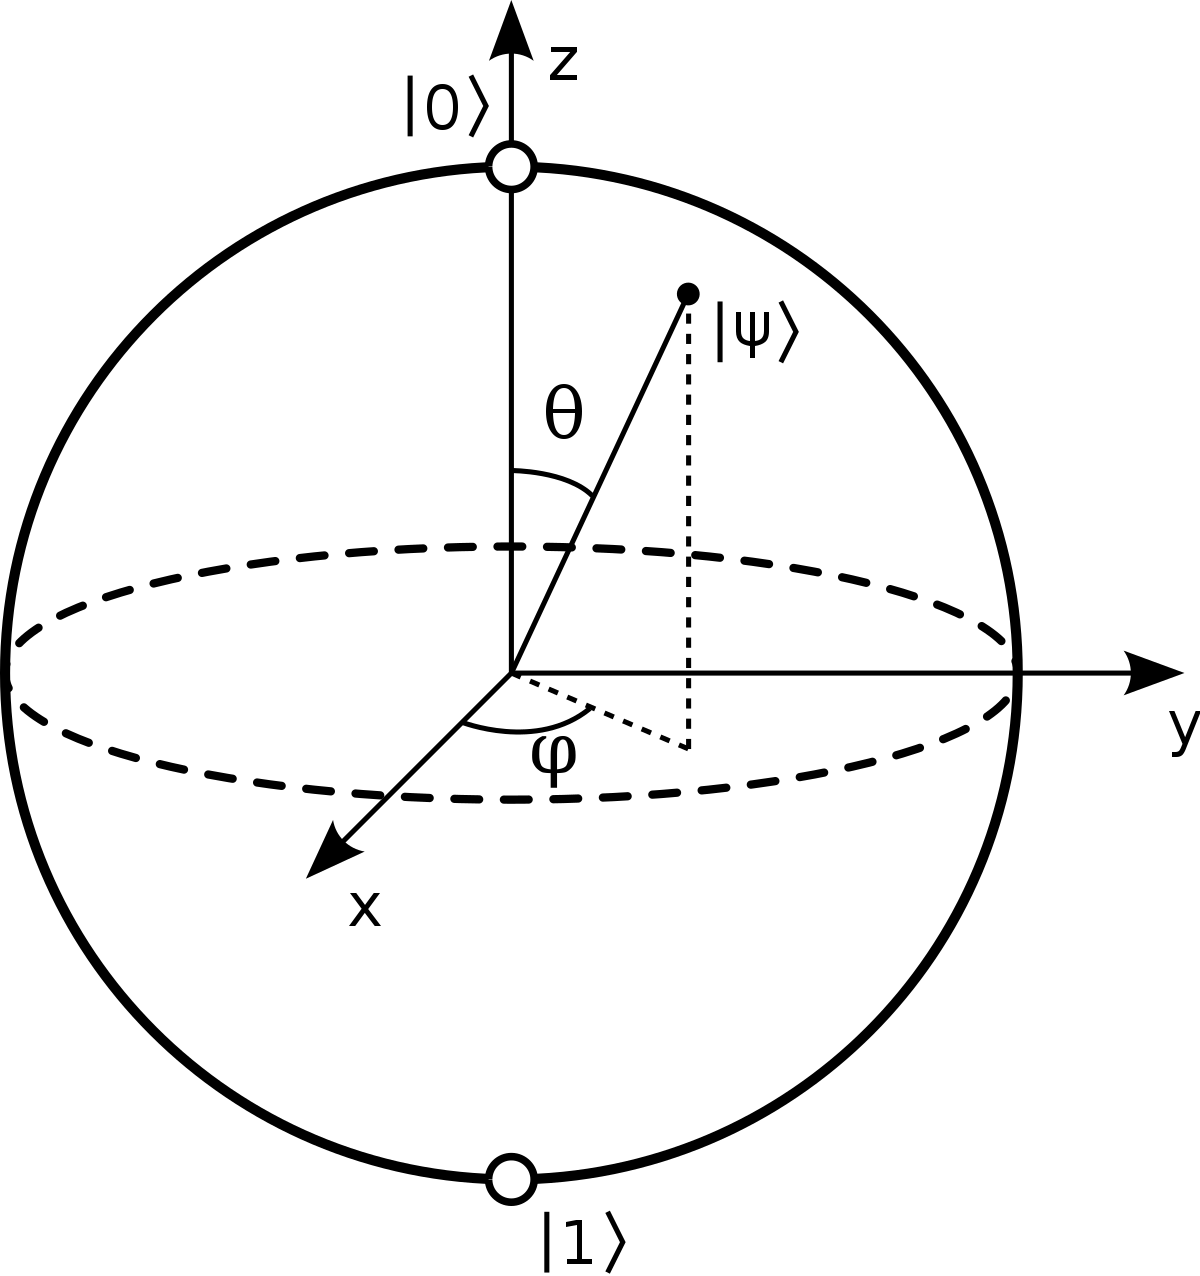
\includegraphics[width = \linewidth]{Chapter 4/4.6.png}
    \caption{The Bloch Sphere}
    \label{fig:my_label}
\end{figure}

Note that the angles $\theta$ and $\phi$ are referring to the angles that the bloch vector $(n_x, n_y, n_z)$ are making, not the qubit itself. Now, to perform a rotation $R_n(\alpha)$ we follow the following procedure:
1. Rotation around Z by $\frac{\pi}{2} - \phi$
2. Rotation around X by $\theta$
3. Rotation around Z by $\alpha$
4. Rotation around X  by $-\theta$
5. Rotation around Z by $\phi - \frac{\pi}{2}$


So we need to show that this procedure is equivalent to $R_n(\alpha)$. We know that:
$$R_n(\alpha) \equiv \cos(\frac{\theta}{2})I - i\sin(\frac{\theta}{2})(n_xX + n_yY + n_zZ)$$
And we must show that this equals our rotation procedure which can be written like so:
$$\left[ \cos\left( \frac{\pi /2 - \phi}{2}\right)I + i\sin\left( \frac{\pi /2 - \phi}{2}\right) Z \right]\left[ \cos\left( \frac{\theta}{2}\right)I +  i\sin\left( \frac{\theta}{2}\right) X \right]$$
$$\left[ \cos\left( \frac{\alpha}{2}\right)I - i\sin\left( \frac{\alpha}{2}\right) Z \right]\left[ \cos\left( \frac{\theta}{2}\right)I - i\sin\left( \frac{\theta}{2}\right) X \right]\left[ \cos\left( \frac{\pi /2 - \phi}{2}\right)I - i\sin\left( \frac{\pi /2 - \phi}{2}\right) Z \right]$$
While it seems tedious to multiply out, we can make the process easier by first multiplying the middle three rotational terms. 
$$\left[ \cos\left( \frac{\theta}{2}\right)I + i\sin\left( \frac{\theta}{2}\right) X \right]\left[ \cos\left( \frac{\alpha}{2}\right)I - i\sin\left( \frac{\alpha}{2}\right) Z \right]$$
$$\left[ \cos\left( \frac{\theta}{2}\right)I - i\sin\left( \frac{\theta}{2}\right) X \right]= \cos\left(\frac{\alpha}{2} \right )I - i\sin\left(\frac{\alpha}{2} \right )n_zZ - i\sin\left(\frac{\alpha}{2} \right ) \sqrt{n_y^2 + n_x^2}Y$$
Now we multiply this with the first and last terms of our rotation procedure like so:
$$\left[ \cos\left( \frac{\pi /2 - \varphi}{2}\right)I + i\sin\left( \frac{\pi /2 - \varphi}{2}\right) Z \right]$$
$$\left[  \cos\left(\frac{\alpha}{2} \right )I - i\sin\left(\frac{\alpha}{2} \right )n_{zZ}- i\sin\left(\frac{\alpha}{2} \right ) (n_y^2 + n_z^2)Y \right]\left[ \cos\left( \frac{\pi /2 - \varphi}{2}\right)I - i\sin\left( \frac{\pi /2 - \varphi}{2}\right) Z \right]$$
Simplifying this out we get,
$$\cos\left(\frac{\alpha}{2} \right )I - i\sin\left(\frac{\alpha}{2} \right )n_zZ- i\sin\left(\frac{\alpha}{2} \right ) \sqrt{n_y^2 + n_x^2}(\frac{n_y}{\sqrt{n_x^2 + n_y^2}}Y + \frac{n_x}{\sqrt{n_x^2 + n_y^2}}X)$$
$$= \cos\left(\frac{\alpha}{2} \right )I - i\sin\left(\frac{\alpha}{2} \right )(n_xX + n_yY + n_zZ)$$
And we have proven that $$R_n(\alpha)$$ indeed is equivalent to a rotation of $$\alpha$$ radians around the $$(n_x, n_y, n_z)$$ axis.


\paragraph{4.7} \textbf{Show that } $XYX = -Y$
\\
$$XYX = \begin{bmatrix} 0& 1\\1 & 0 \end{bmatrix} \begin{bmatrix} 0& i\\-i & 0 \end{bmatrix} \begin{bmatrix} 0& 1\\1 & 0 \end{bmatrix}$$
$$= -\begin{bmatrix} 0& i\\-i & 0 \end{bmatrix} = -Y$$
For the second part, 
$$XR_y(\theta)X = X(\cos(\frac{\theta}{2}) I - i\sin(\frac{\theta}{2})Y)X$$
$$= \cos(\frac{\theta}{2})X^2 - i\sin(\frac{\theta}{2})XYX$$
$$= \cos(\frac{\theta}{2})I + i\sin(\frac{\theta}{2})Y = R_y(-\theta)$$

\paragraph{4.8} \textbf{An arbitrary single qubit unitary operator can be written as} $ U \exp{\iota \alpha} R_N (\theta) $

\\

1. 
$$U = e^{i\alpha}R_n(\theta) = e^{i\alpha}e^{-i(\frac{\theta}{2})(n \cdot \sigma)}$$
Considering the adjoint,
$$U^{\dagger} = (e^{i\alpha})^{\dagger}(e^{-i(\frac{\theta}{2})(n \cdot \sigma)})^{\dagger}$$$$= e^{-i\alpha}e^{i(\frac{\theta}{2})(n \cdot \sigma)}$$
Thus,
$$UU^{\dagger} =  I$$


2. 
$$H = R_x(\pi)R_y(\frac{\pi}{2})e^{i\frac{3\pi}{2}} = e^{-i(\frac{\pi}{2})(\frac{(X+Y)}{2})}$$
Thus,
$\alpha = \frac{3\pi}{2}$$,$$\theta = \pi$, $n = 1, \frac{1}{2}, 0$


3. 
$$S = R_x(0)R_y(0)R_z(\frac{\pi}{2})e^{i*0}$$ 
$$ = e^{(-i)(0)(X/2)}e^{(-i)(0)(Y/2)}e^{(-i)(\pi /2)(Z/2)}$$
$$= e^{(-i)(\frac{\pi}{2})(0X + 0Y + (\frac{\pi}{2})Z)}$$
Thus, 
$\theta = \frac{\pi}{2}$
$\alpha = 0$
$n = 0, 0, \frac{1}{2}$

\paragraph{4.9} \textbf{Explain why any single qubit unitary operator may  be written in different form}
\\

$$UU^{\dagger} = U^{\dagger}U = I$$
$$ U = \begin{bmatrix}a & b\\c & d \end{bmatrix}$$
$$ U^{\dagger} = \begin{bmatrix}a^* & c^*\\b^* & d^* \end{bmatrix}$$
$$ UU^{\dagger} = \begin{bmatrix} aa^* + bb^* & (a^{i} + b^{j})\cdot (c^{*^{i}} + d^{*^{j}})\\(c^{i} + d^{j})\cdot (a^{*^{i}} + b^{*^{j}}) & cc^* + dd^* \end{bmatrix}$$
$$= \begin{bmatrix}1 & 0\\0 & 1\end{bmatrix}$$


This means that the rows/columns are orthonormal with each other and each row/column is normal. Now we can consider U in form 4.12. Here the rows are normal because  


$$aa^* + bb^* = e^{i(a-b/2-\delta /2)} e{-i(a-b/2-\delta /2)}cos(\frac{\gamma}{2})^2 + e^{i(a-b/2+\delta /2)} e{-i(a-b/2+\delta /2)}sin(\frac{\gamma}{2})^2$$
$$ = e^0 sin(\frac{\gamma}{2})^2 + e^0 cos(\frac{\gamma}{2})^2 = 1$$
We can use a similar process to show that the rows are orthonormal and that the columns follow the same rules.

\paragraph{4.12} \textbf{Give A,B,C and } $\alpha$ for the Hadamard gate.
\\

$$H = \frac{1}{\sqrt{2}}\begin{bmatrix}1 & 1\\1 & -1\end{bmatrix}$$
We know, from equation 4.12, that:
$$U = \begin{bmatrix}e^{i(\alpha-\beta /2 - \delta /2)}cos(\frac{\gamma}{2}) & -e^{i(\alpha-\beta /2 + \delta /2)}sin(\frac{\gamma}{2})\\e^{i(\alpha+\beta /2 + \delta /2)}sin(\frac{\gamma}{2}) & e^{i(\alpha-\beta /2 + \delta /2)}cos(\frac{\gamma}{2})\end{bmatrix}$$


So we need to find the $\alpha,\beta, \delta$, and $\gamma$ values that give H. Playing around, we realize its best to take care of the $1/\sqrt{2}$ part by giving gamma the value of pi/2. Now we have to focus on the $e^i$… part. Again, just looking at it, it isn’t too hard to see that, if we set $\beta = 0$, we just need to find a good definition of alpha and sigma values. We realize $\alpha = \pi/2$ and $\sigma = \pi/2$ works. Now, according to theorem 4.1, we have:

$$H = e^{i\pi /2}R_z(0)R_y(\pi /2)R_z(\pi /2)$$
From the proof of the theorem, we say that we just need to define $$A = R_z(0)R_y(\pi/4)$$, $$B = R_y(-\gamma/2)R_z(-(\sigma+\beta)/2)$$, and $$C = R_z(\pi/4)$$, and $$\alpha = \pi /2$$. 

\paragraph{4.13} \textbf{Circuit identities}
\\

$$HXH = \frac{1}{\sqrt{2}}\begin{bmatrix}1 & 1\\1 & -1\end{bmatrix}\begin{bmatrix}0 & 1\\1 & 0\end{bmatrix}\frac{1}{\sqrt{2}}\begin{bmatrix}1 & 1\\1 & -1\end{bmatrix}$$
$$= \frac{1}{2}\begin{bmatrix}2 & 0\\0 & -2\end{bmatrix}$$
$$\begin{bmatrix}1 & 0\\0 & -1\end{bmatrix} = Z$$


$$HYH = \frac{1}{\sqrt{2}}\begin{bmatrix}1 & 1\\1 & -1\end{bmatrix}\begin{bmatrix}0 & -i\\i & 0\end{bmatrix}\frac{1}{\sqrt{2}}\begin{bmatrix}1 & 1\\1 & -1\end{bmatrix}$$
$$= \frac{1}{2}\begin{bmatrix}0 & 2i\\-2i & 0\end{bmatrix}$$
$$\begin{bmatrix}0 & i\\-i & 0\end{bmatrix} = -Y$$


$$HZH = \frac{1}{\sqrt{2}}\begin{bmatrix}1 & 1\\1 & -1\end{bmatrix}\begin{bmatrix}1 & 0\\0 & -1\end{bmatrix}\frac{1}{\sqrt{2}}\begin{bmatrix}1 & 1\\1 & -1\end{bmatrix}$$
$$= \frac{1}{2}\begin{bmatrix}0 & 2\\2 & 0\end{bmatrix}$$
$$\begin{bmatrix}0 & 1\\1 & 0\end{bmatrix} = X$$

\paragraph{4.14} \textbf{Show that} $HTH = R_x(\pi/4)$

\\

$$HTH = \frac{1}{\sqrt{2}}\begin{bmatrix}1 & 1\\1 & -1\end{bmatrix}\begin{bmatrix}1 & 0\\0 & e^{i\pi /4}\end{bmatrix}\frac{1}{\sqrt{2}}\begin{bmatrix}1 & 1\\1 & -1\end{bmatrix}$$
$$= \begin{bmatrix}\frac{1}{2} + \frac{1}{2}e^{i \pi /4} & \frac{1}{2} - \frac{1}{2}e^{i \pi /4}\\\frac{1}{2} - \frac{1}{2}e^{i \pi /4} & \frac{1}{2} + \frac{1}{2}e^{i \pi /4}\end{bmatrix}$$


Our goal in the end is to get a matrix that looks like:
$$R_x(\frac{\pi}{4}) = \begin{bmatrix}\cos(\frac{\pi}{8}) & -i\sin(\frac{\pi}{8})\\-i\sin(\frac{\pi}{8}) & \cos(\frac{\pi}{8})\end{bmatrix}$$
This leads us to take out a global phase of $$e^{i\pi /8}$$.
$$HTH = e^{i\pi /8}\begin{bmatrix}\frac{1}{2}e^{-i\pi /8} + \frac{1}{2}e^{i\pi /8} & \frac{1}{2}e^{-i\pi /8} - \frac{1}{2}e^{i\pi /8}\\\frac{1}{2}e^{-i\pi /8} - \frac{1}{2}e^{i\pi /8} & \frac{1}{2}e^{-i\pi /8} + \frac{1}{2}e^{i\pi /8}\end{bmatrix}$$
$$= e^{i\pi /8} \begin{bmatrix}\cos(\frac{\pi}{8}) & -i\sin(\frac{\pi}{8})\\-i\sin(\frac{\pi}{8}) & \cos(\frac{\pi}{8})\end{bmatrix}$$


\paragraph{4.16} \textbf{Matrix representation of multi-qubit gates}
\\

To build the matrix we have to see what the effect of the circuit is on the different computational basis states. For the state $|00> = [1 0][1 0] = [1 0 0 0]$, the circuit changes it to $|0>|+> = [1/\sqrt(2) 1/\sqrt(2) 0 0]$. For the state $|01> = [1 0][0 1] = [0 1 0 0]$, the circuit changes the state to $|0>|-> = [1/\sqrt(2) -1/\sqrt(2) 0 0]$. For the state $|10> = [0 1][1 0] = [0 0 1 0]$, the circuit changes the state to $|1>|+> = [0 0 1/\sqrt(2) 1/\sqrt(2)]$. For the state $|11> = [0 1][0 1] = [0 0 0 1]$, the circuit changes the state to $|1>|-> = [0 0 1/\cite{}sqrt(2) -1/\sqrt(2)]$. 
        Thus, using these results, we can build the following matrix:
                
$$\begin{bmatrix}\frac{1}{\sqrt{2}} & \frac{1}{\sqrt{2}} & 0 & 0 \\
\frac{1}{\sqrt{2}} & -\frac{1}{\sqrt{2}} & 0 & 0 \\
0 & 0 & \frac{1}{\sqrt{2}} & \frac{1}{\sqrt{2}} \\
0 & 0 & \frac{1}{\sqrt{2}} -\frac{1}{\sqrt{2}} \end{bmatrix}$$


Using the same process, for the next circuit we get:


$$\begin{bmatrix}\frac{1}{\sqrt{2}} & 0 & \frac{1}{\sqrt{2}} & 0\\
0 & \frac{1}{\sqrt{2}} & 0 & \frac{1}{\sqrt{2}}\\
\frac{1}{\sqrt{2}} & 0 & -\frac{1}{\sqrt{2}} & 0\\
0 & \frac{1}{\sqrt{2}}& 0 & -\frac{1}{\sqrt{2}} \end{bmatrix}$$        






\paragraph{4.17} \textbf{ Building CNOT from controlled-Z gates}
\\

To construct a CNOT gate from one controlled Z gate, we can use the following circuit:

Apply a Hadamard gate to the first qubit (control qubit)
Apply a Controlled-Z gate with the first qubit as control and the second qubit as target.
Apply a Hadamard gate to the first qubit (control qubit)
The matrix operation of a CNOT gate with the first qubit as the control qubit and the second qubit as the target qubit is given by:

$$\text{CNOT} = \begin{bmatrix}0 & 0 & 0 & 1 \\ 0 & 0 & 1 & 0 \\ 0 & 1 & 0 & 0 \\ 1 & 0 & 0 & 0\end{bmatrix}$$
The matrix operation of a controlled Z gate with the control qubit as the first qubit and the target qubit as the second qubit is given by:

$$\text{CZ} = \begin{bmatrix}1 & 0 & 0 & 0 \\ 0 & 1 & 0 & 0 \\ 0 & 0 & 1 & 0 \\ 0 & 0 & 0 & -1\end{bmatrix}$$

The matrix operation of a Hadamard gate on a single qubit is given by:

$$\text{H} = \frac{1}{\sqrt{2}} \begin{bmatrix}1 & 1 \\ 1 & -1\end{bmatrix}$$

To find the matrix operation of the circuit described, we need to find the matrix product of the individual gates in the order they appear in the circuit.

The matrix operation of the circuit is:
$$\text{CNOT} = \text{H} \cdot \text{CZ} \cdot \text{H}$$

You can use matrix multiplication to find the final matrix representation of the CNOT gate:


As you can see, the matrix representation of the CNOT gate is identical to the one obtained by directly applying a CNOT gate, which means that the circuit constructed using one Controlled-Z gate and two Hadamard gates indeed implements a CNOT gate.


\paragraph{4.18} \textbf{Show that}

\\

For both circuits, their effect on the computational basis states are the same: for $|00> = [1 0 0 0]$, both don’t change it, for $|01> = [0 1 0 0]$, both don’t change it, for $|10> = [0 0 1 0]$, both don’t change it, and finally for $|11> = [0 0 0 1]$, both change this to $[0 0 0 -1]$. Thus, both circuits’ corresponding matrix is:
$$\begin{bmatrix}1 & 0 & 0 & 0 \\
0 & 1 & 0 & 0 \\
0 & 0 & 1 & 0 \\
0 & 0 & 0 & -1\end{bmatrix}$$
Thus, the two circuits are equal.

\paragraph{4.19} \textbf{CNOT action on density matrices}

\\

When a unitary operator is applied to a density operator, it has the effect: Up
Thus, apply $[CNOT(1 \rightarrow 2) p \text{Hermitian}_\text{Conjugate} (CNOT(1 \rightarrow 2))]$, we get:


$$\begin{bmatrix}p_{11} & p_{12} & p_{14} & p_{13} \\
p_{21} & p_{22} & p_{24} & p_{23} \\
p_{41} & p_{42} & p_{44} & p_{43} \\
p_{31} & p_{32} & p_{34} & p_{33}\end{bmatrix}$$

\paragraph{4.20} \textbf{CNOT Basis transformations}
\\

Representing the operators (H1 tensor H2) with the matrix


$$\frac{1}{2}\begin{bmatrix}1 & 1 & 1 & 1 \\
1 & -1 & 1 & -1 \\
1 & 1 & -1 & -1 \\
1 & -1 & -1 & 1\end{bmatrix}$$


and the operator CNOT(2 $\rightarrow$ 1) as 
$$\begin{bmatrix}1 & 0 & 0 & 0\\
0 & 0 & 0 & 1 \\
0 & 0 & 1 & 0 \\
0 & 1 & 0 & 0\end{bmatrix}$$


(based off how it changes the computational basis states), we then multiply matrix (H1 tensor H2) CNOT(2$\rightarrow$1) (H1 tensor H2) to get the matrix 


$$\begin{bmatrix}1 & 0 & 0 & 0\\
0 & 0 & 0 & 1 \\
0 & 0 & 1 & 0 \\
0 & 1 & 0 & 0\end{bmatrix}$$


which is the matrix of the operator CNOT(1 $\rightarrow$ 2). Thus, applying two hadamards, CNOT(2$\rightarrow$1), and again two hadamards is the same as applying CNOT(1$\rightarrow$2).Now, let's say that instead of the computational basis, we are in the $|+>|->$ basis. Lets say the first qubit is the control qubit, and the second is the target. This is the same as the circuit 


(H1 tensor H2) CNOT(2$\rightarrow$1) (H1 tensor H2) 


and with this circuit we get $|0>|0>$ CNOT(2$\rightarrow$1) = $|0>|0>$ (H1 tensor H2) = $|+>|+>$. Using the same process for input qubits $|->|+>, |+>|->$, and $|->|->$, we get the following formulas:


$$|+>|+> ---> |+>|+>$$
$$|->|+> ---> |->|+>$$
 $$|+>|-> ---> |->|->$$
$$|->|-> ---> |+>|->$$

       
        
We notice that it seems that, even though the first qubit is the control and the second is the target, the roles are flipped! Thus, the roles of control and target are ambiguous when qubits are not in the computational basis, or the classical bit basis. You can also tell from the circuit that this flipping of roles happens, because the circuit essentially says that CNOT(2$\rightarrow$1), when hadamard on both sides, is the same as CNOT(1-2), so with any states that can be turned into the computational basis states upon being “hadamarded”(and inversely be turned back) can have CNOT(1$\rightarrow$2) = CNOT(2$\rightarrow$1). These states are the $|+>, |->$ states.


\paragraph{4.21} \textbf{Verify}
\\

Lets go through all cases:
$1, 1, q -> 1, 1,$
\\
$$ V(q) -> 1, 0,$$
$$ V(q) -> 1, 0,$$
$$ V(q) -> 1, 1, $$
$$V(q) -> 1, 1, $$
$$V^2(q) = U(q)$$
$ 1, 0, q -> 1, 0, q -> 1, 1, q -> 1, 1, V_{adjoint}(q) -> 1, 0, V_{adjoint}(q) -> 1, 1, VV_{adjoint}(q) = q$
$0, 1, q -> 0, 1, V(q) -> 0, 1, V(q) -> 0, 1, V_{adjoint} V(q) -> 0, 1, q -> 0, 1, q
0, 0, q -> 0, 0, q -> 0, 0, q -> 0, 0, q -> 0, 0, q -> 0, 0, q$
 
Thus, the figure does indeed implement the a C2(U) circuit.

\paragraph{4.25} \textbf{}
\\

1. Three toffoli gates with the last two bits switching at each gate
\begin{figure}[h!]
    \centering
    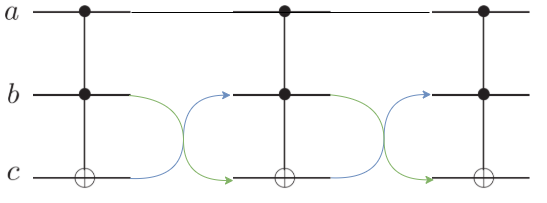
\includegraphics[width = \linewidth]{Chapter 4/4.25.png}
    \caption{4.25 : Three toffoli gates with the last two bits switching at each gate}
    \label{fig:my_label}
\end{figure}

2. We can replace the first and the last toffoli gate like:

\begin{figure}[h!]
    \centering
    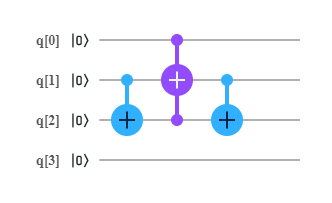
\includegraphics{Chapter 4/4.25(1).png}
    \caption{4.25 : We can replace the first and the last toffoli gate like}
    \label{fig:my_label}
\end{figure}


\paragraph{4.26} \textbf{Show that the circuit}
\\
$$X = \begin{bmatrix} 1 & 0\\0 & 1 \end{bmatrix}$$     $$R_y(\pi /4) = \begin{bmatrix} cos(\pi /8) & -sin(\pi /8)\\cos(\pi /8) & sin(\pi /8) \end{bmatrix}$$     $$R_y(-\pi /4) = \begin{bmatrix} cos(\pi /8) & sin(\pi /8)\\cos(\pi /8) & -sin(\pi /8) \end{bmatrix}$$
We can consider each of the different transformations for the four possible computational basis states of the first two qubits.
1. $$|00\rangle$$ results in $$R_y(\pi /4)R_y(\pi /4)R_y(-\pi /4)R_y(-\pi /4)$$
$$= \begin{bmatrix}1 & 0\\0 & 1\end{bmatrix}$$
2. $$|01\rangle$$ results in $$R_y(\pi /4)XR_y(\pi /4)R_y(-\pi /4)XR_y(-\pi /4)$$
$$= \begin{bmatrix}1 & 0\\0 & 1\end{bmatrix}$$
3. $$|10\rangle$$ results in $$R_y(\pi /4)R_y(\pi /4)XR_y(-\pi /4)R_y(-\pi /4)$$
$$= \begin{bmatrix}-1 & 0\\0& 1\end{bmatrix}$$
4. $$|10\rangle$$ results in $$R_y(\pi /4)XR_y(\pi /4)XR_y(-\pi /4)XR_y(-\pi /4)$$
$$= \begin{bmatrix}0 & 1\\1& 0\end{bmatrix}$$
Which makes sense. You only want to invert the bit when both bits “a” and “b” are 1. 

\paragraph{4.27} \textbf{Using CNOT construct the gate}
\\

The gate implements the following changes to the computational basis states:
$$|000\rangle --> |000\rangle$$
$$|001\rangle --> |111\rangle$$
$$|010\rangle --> |001\rangle$$
$$|011\rangle --> |010\rangle$$
$$|100\rangle --> |011\rangle$$
$$|101\rangle --> |100\rangle$$
$$|110\rangle --> |101\rangle$$
$$|111\rangle --> |110\rangle$$


The circuit will be like:

  $$CNOT q[0], q[1]$$
  $$CNOT q[1], q[2]$$
  $$Toffoli q[0], q[1], q[2]$$
  $$CNOT q[1], q[2]$$
  $$CNOT q[0], q[1]$$

  \begin{figure}
      \centering
      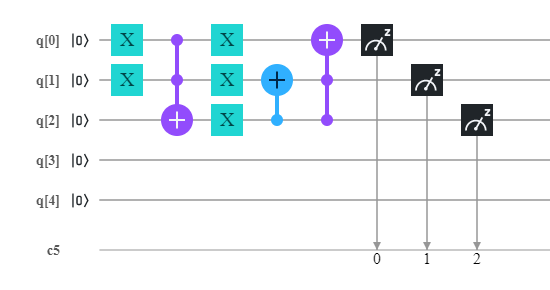
\includegraphics{Chapter 4/4.27.png}
      \caption{}
      \label{fig:my_label}
  \end{figure}

This circuit uses CNOT gates to flip the states of the second and third qubits based on the state of the first qubit, and a Toffoli gate to flip the state of the third qubit based on the states of the first and second qubits. The order of the CNOT and Toffoli gates, as well as the qubits they act on, are chosen so that the overall circuit performs the desired transformations

\paragraph{4.32} \textbf{Density Matrix}
\\

Given that outcome i occurs, the state of the quantum system is: 


  



Thus, if a measurement occurs there is a p(0) chance that outcome 0 occurs and a p(1) chance that outcome 1 occurs. This means that the state will be:


$$p^\prime = p(0)\frac{P_0 \rho P_0}{p(0)} + p(1)\frac{P_1 \rho P_1}{p(1)} = P_0 \rho P_0 + P_1 \rho P_1$$
Now for the second part of the question.
$$\rho = \sum_{i} p_i |\psi_a\rangle |\psi_b\rangle \langle \psi_a |   \langle \psi_b| $$
$$tr_b(\rho) = \sum_{i} p_i tr_b(|\psi_a\rangle |\psi_b\rangle \langle \psi_a |   \langle \psi_b|) $$
$$= \sum_{i} p_i tr_b(|\psi_a\rangle \langle \psi_a | \otimes |\psi_b\rangle \langle \psi_b|) $$$$ = \sum_{i} p_i (|\psi_a\rangle \langle \psi_a |) \langle \psi_b|\psi_b\rangle $$
Finding the trace of the post-measurement (but not post-observation) state,  
$$tr_{b}(\rho^\prime) = \sum_{i} p_i tr_b(P_0|\psi_a\rangle |\psi_b\rangle \langle \psi_a |   \langle \psi_b|P_0) + tr_b(P_1|\psi_a\rangle |\psi_b\rangle \langle \psi_a |   \langle \psi_b|P_1) $$$$tr_{b}(\rho^\prime) = \sum_{i} p_i tr_b(|\psi_a\rangle  \langle \psi_a | \otimes P_0|\psi_b\rangle   \langle \psi_b|P_0) + tr_b(|\psi_a\rangle \langle \psi_a | \otimes P_1|\psi_b\rangle  \langle \psi_b|P_1) $$
$$tr_{b}(\rho^\prime) = \sum_{i} p_i (|\psi_a\rangle  \langle \psi_a |)( \langle \psi_b|P_0|\psi_b\rangle   +\langle \psi_b|P_1|\psi_b\rangle)  $$
$$tr_{b}(\rho^\prime) = \sum_{i} p_i (|\psi_a\rangle  \langle \psi_a |)( \langle \psi_b|(P_0 + P_1)|\psi_b\rangle)  $$
But by the completeness relation we know that   , thus $$tr_b(\rho^\prime) = tr_b(\rho)$$

\paragraph{4.33} \textbf{Measurement in the Bell Basis}

\\

We know that,
$$|00\rangle = \frac{|B_{00}\rangle + |B_{10}\rangle}{\sqrt{2}}$$


If you put the $|00\rangle$ through the circuit, we get $\frac{|00\rangle + |10\rangle}{\sqrt{2}}$ as the result. This means that for $|00\rangle$, the circuit is indeed measuring it with respect to the Bell states. We can confirm that this holds for the other three computational basis states. Now we must show that the measurement is being performed with the projectors onto the Bell states as corresponding POVM elements. To do so, once again consider the computational basis state $|00\rangle$.


If the Bell state of the projectors are the corresponding POVM elements, then the state of $|00\rangle$ after a measurement in the Bell basis would be either 


$$\left(\frac{P_{00}|\psi\rangle}{\sqrt{p(00)}}\right)$$ or$$\left(\frac{P_{10}|\psi\rangle}{\sqrt{p(10)}}\right)$$


Re-normalizing this, we see that the projector tells us the state will be either


$$\frac{|00\rangle + |11\rangle}{\sqrt{2}}$$ or $$\frac{|00\rangle - |11\rangle}{\sqrt{2}}$$, which are exactly the Bell states our circuit predicts. One can go through similar work for the other computational basis states to ensure that the problem statement is indeed correct.


\paragraph{4.34} \textbf{Measuing an Operator}
\\

\begin{figure}[h!]
    \centering
    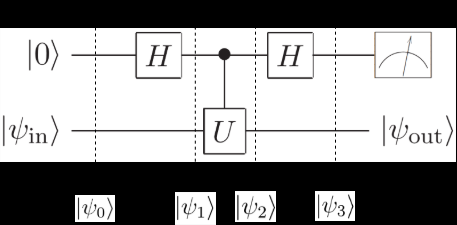
\includegraphics{Chapter 4/4.34.png}
    
    \label{fig:my_label}
\end{figure}

$$|\psi_0\rangle = |0\rangle |\psi_{in}\rangle$$
$$|\psi_1\rangle = \frac{1}{\sqrt{2}}(|0\rangle |\psi_{in} \rangle + |1\rangle |\psi_{in}\rangle)$$
$$|\psi_2\rangle = \frac{1}{\sqrt{2}}(|0\rangle |\psi_{in}\rangle + |1\rangle U|\psi_{in}\rangle)$$
$$|\psi_3\rangle = \frac{1}{2}\left[ (|0\rangle + |1\rangle) |\psi_{in}\rangle + (|0\rangle - |1\rangle)U |\psi_{in}\rangle \right]$$
$$ = \frac{1}{2}\left[|0\rangle (I + U)|\psi_{in}\rangle + |1\rangle (I - U) |\psi_{in}\rangle \right]$$
So if the measurement gives us 0 (representing the +1 eigenvalue), we have the corresponding eigenvector to be $$(I+U)|\psi\rangle$$. This is indeed true, since $$U(I+U)|\psi\rangle = (U+I)|\psi\rangle$$, since U is both hermitian and unitary. 


If the measurement gives us a 1 (representing the -1 eigenvalue), we have $$U(I-U)|\psi\rangle = -1(I-U)|\psi\rangle$$. Thus, we have showed that the circuit implements a measurement of U.  

\paragraph{4.35} \textbf{Measurement commutes with controls}
\\

The figure:
\begin{figure}[h!]
    \centering
    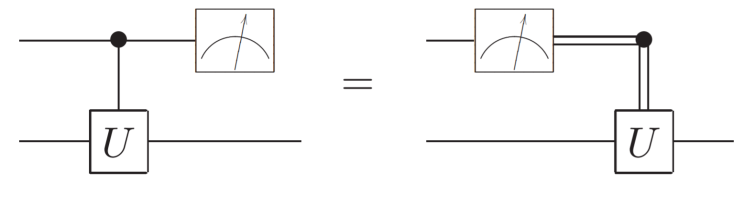
\includegraphics[width = \linewidth]{Chapter 4/4.35.png}
    
    \label{fig:my_label}
\end{figure}

Considering the circuit on the left first, we have:
$$|\psi_0\rangle = (a|0\rangle + b|1\rangle)(c|0\rangle + d|1\rangle)$$
$$|\psi_0\rangle = (ac|0\rangle |0\rangle + ad|0\rangle |1\rangle + bc|1\rangle |0\rangle +bd|1\rangle |1\rangle)$$
$$|\psi_1\rangle = (ac|0\rangle |0\rangle + ad|0\rangle |1\rangle + (bc)U|1\rangle |0\rangle +(bd)U|1\rangle |1\rangle)$$
After measurement, the state of the 2nd qubit becomes 
$$a(c|0\rangle + d|1\rangle ) + b(cU|0\rangle + dU|1\rangle )$$


Considering the circuit on the right, if the first qubit is $$|0\rangle$$ then the second qubit is $$c|0\rangle + d|1\rangle $$. Likewise, if the first qubit is $$|1\rangle$$, then the second qubit is $$cU|0\rangle + dU|1\rangle $$. Thus, combining the two facts, we get $$a(c|0\rangle + d|1\rangle ) + b(cU|0\rangle + dU|1\rangle )$$ and both circuits are equivalent.


\paragraph{4.36} \textbf{Construct a Quantum Circuit}
\\

In this figure, q[0] is the first qubit of the first number, q[1] is the first qubit of the 2nd number, q[2] is the 2nd qubit of the first number, and q[3] is the 2nd qubit of the 2nd number. Note that the pauli-x matrices in the beginning are just to define the initial values of the 2 numbers. 

 \begin{figure}[h!]
     \centering
     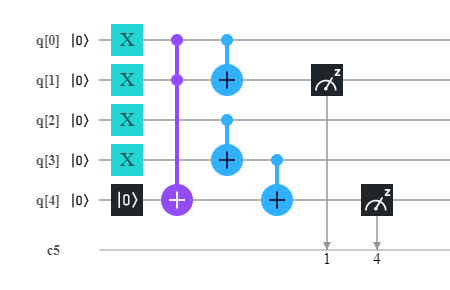
\includegraphics{Chapter 4/4.36.png}
     
     \label{fig:my_label}
 \end{figure}


\paragraph{4.37} \textbf{Provide a decomposition}
\\

Using the process in the lesson we initially get,
$$U_3U_2U_1U = \begin{bmatrix}1 & 0 & 0 & 0 \\0 & i\frac{\sqrt{2}}{2} & 0 & -i\frac{\sqrt{2}}{2} \\0 & \frac{1}{\sqrt{2}} & 0 & \frac{1}{\sqrt{2}} \\0 & 0 & 1 & 0 \end{bmatrix}$$
$$U_1 = \begin{bmatrix}1 & 0 & 0 & 0 \\0 & \frac{1}{\sqrt{2}} & 0 & -\frac{1}{\sqrt{2}} \\0 & 0 & 1 & 0 \\0 & \frac{1}{\sqrt{2}} & 0 & \frac{1}{\sqrt{2}} \end{bmatrix}$$ 

$$U_2 = \begin{bmatrix} \frac{1}{\sqrt{2}}& 0 & \frac{1}{\sqrt{2}} & 0 \\
0 & 1 & 0 & 0 \\
\frac{1}{\sqrt{2}} & 0 & -\frac{1}{\sqrt{2}} & 0 \\
0 & 0 & 0 & 1 \end{bmatrix}$$ 

$$U_3 = \begin{bmatrix} \frac{1}{\sqrt{2}}& 0 & 0 & \frac{1}{\sqrt{2}} \\
0 & 1 & 0 & 0 \\
0 & 0 & 1 & 0 \\
\frac{1}{\sqrt{2}} & 0 & 0 & -\frac{1}{\sqrt{2}} \end{bmatrix}$$
This means that 
$$U_4 = \begin{bmatrix}1 & 0 & 0 & 0 \\
0 & -i\frac{\sqrt{2}}{2} & \frac{1}{\sqrt{2}} & 0 \\
0 & 0 & 0 & 1 \\
0 & i\frac{\sqrt{2}}{2} & \frac{1}{\sqrt{2}} & 0 \end{bmatrix}$$ 
Except, this matrix isn’t a two-level unitary matrix. We can still decompose it into two-level unitary matrices, with a similar process such that


$$V_2V_1U_4 = I$$
$$V_1 = \begin{bmatrix}1 & 0 & 0 & 0 \\
0 & i\frac{\sqrt{2}}{2} & 0 & -i\frac{\sqrt{2}}{2} \\
0 & 0 & 1 & 0 \\
0 & \frac{1}{\sqrt{2}} & 0 & \frac{1}{\sqrt{2}} \end{bmatrix}$$   

$$U_4 = V_1^{\dagger} V_2^{\dagger}$$
$$U_4U_3U_2U_1U = I$$
$$V_1^{\dagger} V_2^{\dagger}U_3U_2U_1U = I$$



Thus, the final two-level unitary decomposition is $$U = U_1^{\dagger}U_2^{\dagger}U_3^{\dagger}V_2V_1$$

\paragraph{4.39} \textbf{Find a Quantum Circuit}
\\

In this two-level unitary matrix, it only acts on the vector components $$|010\rangle$$ to $$|111\rangle$$. The corresponding circuit is shown above.

\begin{figure}[h!]
    \centering
    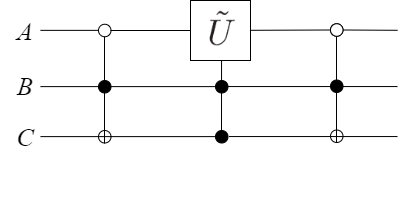
\includegraphics{Chapter 4/4.39.png}
    
    \label{fig:my_label}
\end{figure}


\paragraph{4.40} \textbf{Arbitrary } $\alpha $ and $\beta$
\\
$$E(R_{^{n}}(\alpha), R_{^{n}}(\alpha+\beta)) = ||(R_{^{n}}(\alpha) - R_{^{n}}(\alpha+\beta))|\psi\rangle|| = \sqrt{\langle \psi |(R_{^{n}}(\alpha) - R_{^{n}}(\alpha+\beta))^{\dagger}(R_{^{n}}(\alpha) - R_{^{n}}(\alpha+\beta))|\psi \rangle }$$

$$R_{^{n}}(\alpha) \equiv \exp(-i\alpha^{n}\cdot {\sigma}/2) = \cos(\frac{\alpha}{2})I - \iota \sin(\frac{\alpha}{2})(n_{xX} + n_{yY} + n_{zZ})$$


To simplify the calculations, use the following substitutions:
$$d = cos(\frac{\alpha}{2}) - cos(\frac{\alpha + \beta}{2})$$
$$f = sin(\frac{\alpha}{2}) - sin(\frac{\alpha + \beta}{2})$$


$$(R_{^{n}}(\alpha) - R_{^{n}}(\alpha+\beta))^{\dagger}(R_{^{n}}(\alpha) - R_{^{n}}$$
$$(\alpha+\beta)) = (dI - if(n_xX+n_yY+n_zZ))(dI + if(n_xX+n_yY+n_zZ)) = (d^2I+if(n_xX+n_yY+n_zZ)^2)$$
So now we know that the desired value is 


$$\langle \psi |(d^2I+if(n_xX+n_yY+n_zZ)^2)|\psi \rangle = d^2 + \langle \psi | f(n_xX+n_yY+n_zZ)^2 |\psi \rangle$$


Now remember that  $$\langle \psi |AA| \psi \rangle = ||A|\psi \rangle||^2$$. So in order to calculate $$\langle \psi | f(n_xX+n_yY+n_zZ)^2 |\psi \rangle$$, we just have to find $$|| (n_xX+n_yY+n_zZ) |\psi \rangle||$$ (remember that f and ni are real, and X, Y, and Z are Hermitian). Letting


$$|\psi \rangle = \begin{bmatrix}a 
b\end{bmatrix}$$
$$(n_xX+n_yY+n_zZ) |\psi \rangle = \begin{bmatrix}(n_xb - n_ybi + n_za) 
(n_xa+n_yai - n_zb) \end{bmatrix}$$


So the magnitude of this vector equals:


$$|n_xb - n_ybi + n_za|^2 + |n_xa+n_yai - n_zb|^2 = |(n_xb + n_za) - (n_yb)i|^2 + |(n_xa - n_zb) + (n_ya)i|^2$$


Expanding out, and using $$a^2 + b^2 = 1$$ and $$n_x^2 + n_y^2 + n_z^2 = 1$$, we find that the magnitude of the above vector is 1. Thus, $$\langle \psi | f(n_xX+n_yY+n_zZ)^2 |\psi \rangle$$ is equal to $$f^2$$. Thus we have,  


$$ ||(R_{\^{n}}(\alpha) - R_{\^{n}}(\alpha+\beta))|\psi\rangle|| = \sqrt{d^2 + f^2}$$


$$\sqrt{\left[ cos(\frac{\alpha}{2}) - cos(\frac{\alpha + \beta}{2}\right]^2 \left[ sin(\frac{\alpha}{2}) - sin(\frac{\alpha + \beta}{2}\right]^2}$$
$$= \sqrt{2-2\left( cos(\frac{\alpha}{2})cos(\frac{\alpha + \beta}{2} - sin(\frac{\alpha}{2})sin(\frac{\alpha + \beta}{2}) \right)}$$
Remember that, 
$$cos(\frac{\alpha + \beta}{2} - \frac{\alpha}{2}) = cos(\frac{\alpha}{2})cos(\frac{\alpha + \beta}{2} - sin(\frac{\alpha}{2})sin(\frac{\alpha + \beta}{2})$$


Thus, we get a final answer of $$\sqrt{2-2cos(\frac{\beta}{2})}$$, which is equal to the $$|1-exp(i\beta /2)|$$ in the problem statement.


\paragraph{4.41} \textbf{Construction showing the circuit}
\\

Considering the diagram in the question


$$|\psi_0 \rangle = |0\rangle |0\rangle |\psi \rangle  $$
$$|\psi_1 \rangle = \frac{1}{2}(|00\rangle + |01\rangle + |10\rangle + |11\rangle)|\psi \rangle$$
$$|\psi_2 \rangle = \frac{1}{2}(|00\rangle S|\psi \rangle + |01\rangle S|\psi \rangle + |10\rangle S|\psi \rangle + |11\rangle XSX|\psi \rangle)$$
$$|\psi_3 \rangle = \frac{1}{4}(|00\rangle (3S + XSX) |\psi \rangle + |01\rangle (S-XSX)|\psi \rangle + |10\rangle (-S-XSX)|\psi \rangle + |11\rangle (-S+XSX)|\psi \rangle)$$
Considering the $$|00\rangle$$ term, the matrix in front of it can be written as:


$$\frac{\sqrt{10}}{e^{\frac{i\pi}{4}}} \begin{bmatrix} e^{i(\alpha-\frac{\pi}{4})}& 0\\0 & e^{i(\frac{\pi}{4} - \alpha)}\end{bmatrix}$$, $$sin(\alpha) = \frac{1}{\sqrt{10}}$$, $$cos(\alpha) = \frac{3}{\sqrt{10}}$$,
$$p(|00\rangle) = \left| \frac{\sqrt{10}}{4e^{i\frac{\pi}{4}}} \right|^2 = 5/8$$
With some basic trigonometry, we can prove that this matrix is indeed the rotation around the z-axis by theta.


\paragraph{4.42} \textbf{Irrationality of } $\theta$

\\
(1) If $\theta$ is a rational multiple of $2\pi$ ($\theta = 2\pi k$), then there must exist an integer $m$ such that $mk$ is an integer and thus,
$$e^{i(2\pi mk)} = 1$$ 
And so,
$$e^{i(2\pi mk)} = \frac{(3+4i)^m}{5^m} = 1$$, 
$$(3+4i)^m = 5^m$$.


(2) To show this equivalence, all we need to show is that $$(3+4i)^2 \equiv 3+4i (mod 4)$$, and since m is an integer, the rest follows. Expanding out, we see that this equation is true. This means that (3+4i) cannot be a multiple of 5, and thus can never equal $$5^m$$.


\paragraph{4.43} \textbf{Use the result of the previous exercise}
\\
Because $\theta$ is an irrational multiple of $2\pi$, we can use equation 4.76 and show that any single qubit gate in the form $R_z(\alpha)$ can be represented within an error of $\frac{\epsilon}{3}$. Now, we will show that $$HR_z(\alpha)H = R_x(\alpha)$$.
$$R_z(\alpha) = cos(\frac{\alpha}{2})I - isin(\frac{\alpha}{2})(Z)$$
$$HR_z(\alpha)H = H \left[ cos(\frac{\alpha}{2})I - isin(\frac{\alpha}{2})(Z) \right] H$$
$$= cos(\frac{\alpha}{2})I -isin(\frac{\alpha}{2}) HZH$$.
Remember that $H^2 = I$, and that $HZH = X$, so:
$$HR_z(\alpha)H =  cos(\frac{\alpha}{2})I -isin(\frac{\alpha}{2})X = R_x(\alpha)$$
Following the same logic from page 197 (10th anniversary edition), we can approximate any m gate quantum circuit. 

\paragraph{4.44} \textbf{Show the three qubit gate}
\\

$$i = e^{i\frac{\pi}{2}}$$ is just a global phase factor, so the work is the same as the exercise above.

\paragraph{4.45} \textbf{U is unitary}
\\

The statement is easy to see if you write out the H, S, CNOT, and Toffoli Matrices
$$H = \frac{1}{\sqrt{2}} \begin{bmatrix}1 & 1\\
1 & -1\end{bmatrix}$$
$$S = \begin{bmatrix}1 & 0\\0 & i\end{bmatrix}$$
$$CNOT = \begin{bmatrix}1 & 0 & 0 & 0\\0 & 1 & 0 & 0 \\
0 & 0 & 0 & 1 \\
0 & 0 & 1 & 0\end{bmatrix}$$
(Toffoli gate has similar structure as CNOT Gate)


Inspecting these matrices, it’s clear that all four satisfy the conditions stated in the problem. Now we just need to show that any unitary transform constructed by these four gates satisfies the conditions. Any transform can be constructed by using the tensor product or matrix multiplication operation between these four matrices and the identity matrix (which also satisfies the problem’s properties). When we multiply or tensor product, it is clear that all elements remain complex integers and the only scalar coefficient will be in the form:


$$\left( \frac{1}{\sqrt{2}}\right) ^k  = 2^{-k/2}$$

\paragraph{4.46} \textbf{Exponential complexity growth of quantum systems}
\\

$$\rho = \sum_{i} p_i |\psi_n \rangle \ldots |\psi_1 \rangle \otimes \langle \psi_n | \ldots \langle \psi_1 |$$
Each $|\psi_i \rangle$ has dimension 2, so $|\psi_n \rangle \ldots |\psi_1 \rangle$ has dimension $2^n$, and the matrix $\rho$ has dimension $2^n \times 2^n$. Since it’s normalized, the matrix requires $4^n - 1$ independent real numbers to describe it.


\paragraph{4.47} \textbf{Prove the following}
\\
To prove this, all we have to show is that $$e^{A+B} = e^Ae^B if AB = BA$$. To do this, we use


$$e^X = \sum_{i=0}^{\infty}\frac{x^i}{i!}$$
$$e^Ae^B = (\frac{I}{0!} + \frac{A^1}{1!} + \frac{A^2}{2!} \ldots)(\frac{I}{0!} + \frac{B^1}{1!} + \frac{B^2}{2!} \ldots)$$
$$e^{A+B} = (\frac{I}{0!} + \frac{(A+B)^1}{1!} + \frac{(A+B)^2}{2!} \ldots)$$


The nth term in the $e^{A+B}$ expansion is $\frac{(A+B)^n}{n!}$, and if $AB = BA$ is true, we can use the binomial theorem


$$\frac{(A+B)^n}{n!} = \sum_{i=0}^{n} \frac{1}{i!(n-i)!}A^iB^{n-i} = \sum_{i=0}^{n} \left( \frac{A^i}{i!}\right) \left( \frac{B^{n-i}}{(n-i)!}\right) $$
This right hand side is precisely what you get when expanding $e^Ae^B$. In this expansion there is precisely one $$ \left( \frac{A^i}{i!}\right) \left( \frac{B^{n-i}}{(n-i)!}\right)$$ for a specific $n$ and $i$. To complete this question, we need to show that the term $$ \left( \frac{A^i}{i!}\right) \left( \frac{B^{n-i}}{(n-i)!}\right)$$ does not repeat for each $n$. However, this is obvious that for two different $n_1$ and $n_2$ that term cannot repeat, and we are done.


\paragraph{4.48} \textbf{Restriction of } $H_k$
\\
$$c{n \choose c} \leq n^c$$ which is a polynomial in n. 

\paragraph{4.49} \textbf{Baker–Campbell–Hausdorf formula}
\\
Proving equation 4.103:
$$e^{i(A+B)\delta t} = e^{iA\delta t}e^{iB\delta t} + O(\delta t^2)$$
Start similarly to the proof of Trotter Formula.
$$e^{i(A+B)\delta t} = I + \frac{i(A+B)\delta t}{1} + \frac{[i(A+B)]^2\delta t^2}{2!} + O(t^3)$$
$$e^{iA\delta t}e^{iB\delta t} = (I + \frac{iA\delta t}{1} + \frac{(iA)^2\delta t^2}{2!} + O(\delta t^3) )(I + \frac{iB\delta t}{1} + \frac{(iB)^2\delta t^2}{2!} + O(\delta t^3)$$
$$= I + \frac{[i(A+B)]\delta t}{1} + \frac{((iA)^2 + (iB)^2)}{2!} + (iA)(iB)\delta t^2 + O(\delta t^3)$$
In order for this to equal $$e^{i(A+B)\delta t}$$, we need to add the $$O(\delta t^2)$$ term, and we are done.


Proving equation 4.104:
$$e^{iA\delta t/2}e^{iB\delta t}e^{iA\delta t/2} = \left(I + \frac{iA\delta t}{2} + \frac{1}{2!}\left(\frac{iA\delta t}{2} \right)^2 + O(\delta t^3)\right) \left(I + iB\delta t + \frac{1}{2!}(iB\delta t)^2 + O(\delta t^3)\right)$$ 
$$ \left(I + \frac{iA\delta t}{2} + \frac{1}{2!}\left(\frac{iA\delta t}{2} \right)^2 + O(\delta t^3)\right) $$ 
$$= I + i(A+B)\delta t + \frac{(iA + iB)^2 \delta t^2}{2} + O(\delta t^3)$$.


Proving equation 4.105:

\paragraph{4.50} \textbf{}
\\

Part A):
The key is to use equation 4.104, and generalize it with multiple variables.
$$e^{i(A+B)\Delta t} = e^{iA\Delta t/2}e^{iB\Delta t}e^{iA\Delta t/2} + O(\Delta t^3)$$
$$e^{i(C+(A+B))\Delta t} = e^{iC\Delta t/2}e^{i(A+B)\Delta t}e^{iC\Delta t/2} + O(\Delta t^3)$$
$$= e^{iC\Delta t/2} e^{iA\Delta t/2}e^{iB\Delta t}e^{iA\Delta t/2}e^{iC\Delta t/2} + O(\Delta t^3)$$
Thus,
$$e^{-2iH\Delta t}= e^{-i(2H_1 + \ldots 2H_L)} = e^{-iH_1\Delta t}\ldots e^{-iH_{L-1}\Delta t} e^{-2iH_L \Delta t}e^{-iH_{L-1}\Delta t}\ldots e^{-iH_{1}\Delta t} $$
But by exercise 4.47,
$$e^{-2iH_L \Delta t} = e^{-iH_L\Delta t}e^{-iH_L\Delta t}$$
And we are done. 


Part B):
$$E(U_{\Delta t}, e^{-2iH\Delta t}) = max ||(U-V)|\psi \rangle || = O(\Delta t^3)$$
By equation 4.63, 
$$E(U_{\Delta t}^m, e^{-2miH\Delta t})= mO(\Delta t^3)$$
By definition of big O, $$O(\Delta t^3) = \alpha \Delta t^3$$, so we are done.
